\documentclass{article}
\usepackage{xcolor}
\usepackage{tikz-cd}
\usepackage{amsmath}
\usepackage{amssymb}
\usepackage{amsthm}
\usepackage{enumitem}
\usepackage{mathtools}
\usepackage{graphicx}
\usepackage{wrapfig}
\usepackage{tikz}
\usetikzlibrary{arrows}
\usepackage[a4paper, total={6in, 8in}]{geometry}

% environments
\theoremstyle{definition}
\newtheorem*{definition}{Definition}
\newtheorem*{example}{Example}
\newtheorem{exercise}{Exercise}

\theoremstyle{plain}
\newtheorem{theorem}{Theorem}[section]
\newtheorem{corollary}[theorem]{Corollary}
\newtheorem{proposition}{Proposition}[section]
\newtheorem{lemma}{Lemma}[section]

\theoremstyle{remark}
\newtheorem*{remark}{Remark}
\newtheorem*{fact}{Fact}

\newenvironment{claim}[1]{\par\underline{Claim:}\space#1}{\par\smallskip}
\newenvironment{acase}[1]{\par\underline{Case\space#1:}\space}{\par\smallskip}
\newcommand{\astep}[2]{\par\textbf{Step #1: #2}\par\smallskip}

\numberwithin{equation}{section}
% commands
\newcommand{\contra}{\Rightarrow\!\Leftarrow}

\newcommand{\integer}{\mathbb{Z}}
\newcommand{\ratio}{\mathbb{Q}}
\newcommand{\real}{\mathbb{R}}
\newcommand{\complex}{\mathbb{C}}

\newcommand{\rangewith}[4]{{#2}#1{#3}, \cdots, {#2}#1{#4}}
\newcommand{\funtyp}[3]{#1: & #2 & \rightarrow & #3 \\ }
\newcommand{\fundecl}[2]{& #1 & \mapsto & #2 \\ }

\title{Decision algorithm for roots of 2-step}
\author{Junho Lee}

\begin{document}
\pagecolor{white}
\color{black}
\maketitle

\section{General Problem statement}

Given a rational number $\lambda = -u^2$ and fixed $k$ (or number of steps),
one is to determine if $u$ is a root of chebyshev polynomial $s^\mathbf{n}_k(u)$ for some sequence $\mathbf{n}$.

Our goal here is to establish a decision algorithm for such "relational numbers within fixed steps".

\section{Directions given by Professor Hyuk Kim}

The crucial part is to reduce the number of candidates $\mathbf{n}$ to be finite,
so that it could be checked by computation.

The baseline approach is to observe that when $n_1, n_2, \cdots, n_k \to \infty$,
the leading term of increases faster than any other terms,
so that all the solutions converge to $0$.

For instance, in the case of 1-step polynomial we have the one solution
\begin{equation}\label{eqn:1stepsol}
  \lambda = \frac{n_1 + n_3}{n_1 n_2 n_3} \to 0
\end{equation}
as $n_1, n_2, n_3 \to \infty$.

For computation, we need the specific bound.
In this case, we can obtain this as following:
Suppose $n_1, n_2, n_3 > N$. Then,
\[
  \frac{1}{n_2} (\frac{1}{n_1} + \frac{1}{n_3}) < \frac{2}{N^2}
\]

\begin{figure}[h!]
  \centering
  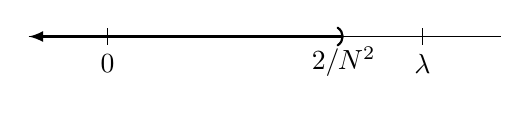
\begin{tikzpicture}
    \draw[] (-3, 0) -- (3, 0);
    \draw[] (-2, 3pt) -- (-2, -3pt) node[below]{$0$};
    \draw[{latex-)}, thick] (-3, 0) -- (1, 0) node[below]{$2 / N^2$};
    \draw[] (2, 3pt) -- (2, -3pt) node[below]{$\lambda$};
  \end{tikzpicture}
\end{figure}

Taking $N$ big enough so that $\frac{2}{N^2} \leq \lambda$,
contradiction can be obtained.
Thus, one of $n_1, n_2, n_3$ should be smaller than $\frac{2}{N^2}$.
We can proceed similarly and give bound to two of the $n_1, n_2, n_3$,
then the other is uniquely decided from (\refeq{eqn:1stepsol}), as $\lambda$ is fixed here.

As such, we can use the limiting behavior of the polynomial to computationally decide
if certain number is a root of chebyshev polynomial of specific degree.

\newpage

\section{My approach for 2-step polynomials}

Will discuss $s_6$ case here.

Recall that
\[
  s^\mathbf{n}_6(u) = n_1 n_2 n_3 n_4 n_5 u^5
  - (n_1 n_2 n_3 + n_1 n_2 n_5 + n_1 n_4 n_5 + n_3 n_4 n_5) u^3
  + (n_1 + n_3 + n_5) u.
\]
and by setting $m_i = \frac{1}{n_i n_{i+1}}$, we get
\[
  \frac{s_6(u)}{n_1 n_2 n_3 n_4 n_5} = u \cdot (u^4 - (m_1 + m_2 + m_3 + m_4) u^2 + (m_1 m_3 + m_1 m_4 + m_2 m_4)).
\]

Hence, for nonzero roots $u$, $\mu := -\lambda = u^2$ is a root of
\[
  P(x) = x^2 - (m_1 + m_2 + m_3 + m_4) x + (m_1 m_3 + m_1 m_4 + m_2 m_4).
\]
The idea is from the observation that \textit{the $m_i$'s only accumulation point is around $0$.}
We will give lower bounds to 3 $m_i$'s, so that the other $m_j$ is determined.
Then, there are only finitely many corresponding $n_i$'s possible,
from which we can decide existence of such a polynomial.

\subsection{First bounds: $m_2$ and $m_3$}

We may assume $\mu > 0$ by a property of relation numbers.
Meanwhile, $P(x)$ can be reformulated to
\[
  P(x) = (x - m_1 - m_2) (x - m_3 - m_4) - m_2 m_3 = 0
\]
so that the following can be obtained.
\[
  \lvert \mu - (m_1 + m_2) \rvert \cdot \lvert \mu - (m_3 + m_4) \rvert = \lvert m_2 m_3 \rvert
\]

Recall that $m_i = 1 / (n_i n_{i+1})$, hence being a reciprocal of an integer.
Specifically,
\[
  \mu - (m_1 + m_2) \in
  R_\mu := \left\{ \mu - \frac{1}{k_1} - \frac{1}{k_2} \; \middle\vert \; k_1, k_2 \in \integer \right\}.
\]
Thus, $\lvert m_2 m_3 \rvert \in R_\mu \cdot R_\mu$,
from which one could deduce
\[ \lvert m_2 m_3 \rvert \geq \min \lvert R_\mu \cdot R_\mu \rvert = \min(R_\mu)^2. \]

To use this inequality, we need to show that $0$ is not an accumulation point of $R_\mu$.

\begin{proposition}
  All accumulation points of $U := \{ \frac{1}{k_1} + \frac{1}{k_2} \mid k_1, k_2 \in \integer \}$
  are $0$ or $T := \{ \frac{1}{N} \mid N \in \integer \}$.
\end{proposition}
\begin{proof}
  It is easy to check that accumulation points inside $U$ is in $T$.
  Outside $U$, any accumulation points should be in $\bar{U}$.
  Consider $f : [0, 1]^2 \to \real$ given by $f(x, y) = x + y$.
  Since $U = f(T^2)$ and $\overline{T^2}$ is a closed set inside compact $[0,1]^2$,
  \[ \bar{U} = f(\overline{T^2}) = f((\bar{T})^2) = f((\{ 0 \} \cup T)^2) \]
  by property of product topology.
  Thus, $\bar{U} = \{ 0 \} \cup T \cup U$, so there is no accumulation point outside $T$.
\end{proof}

By the above proposition,
$0$ cannot be an accumulation point of $R_\mu$ if $\mu \notin T$.
Note that if $\mu \in T$, $\mu$ is a root of 1-step polynomial anyway.
Thus, we may only consider the case where $\mu \notin T$,
so there are only finitely many of $R_\mu$ around $0$.
Consequently,
\[
  \lvert m_2 m_3 \rvert \geq L := \min(R_\mu)^2 > 0
\]
which is a meaningful bound.

Then, the lower bound $\lvert m_2 m_3 \rvert \geq L$
gives bounds on both $m_2$ and $m_3$.
In particular, we know $\lvert m_2 \rvert, \lvert m_3 \rvert \leq 1$,
so $\lvert m_2 \rvert \geq L$ and the same holds for $m_3$ as well.

This bounds let us to choose and fix $m_2 := a_2$ and $m_3 := a_3$, so that only $m_1$ and $m_4$ are remaining.

\subsection{Remaining bounds}

Let us get our focus back into this (updated) formula.
\[
  \lvert \mu - (m_1 + a_2) \rvert \cdot \lvert \mu - (a_3 + m_4) \rvert = \lvert a_2 a_3 \rvert
\]
Some balancing is needed here:
\[
  A_\mu (m_1) \cdot B_\mu (m_4)
  := \left\lvert 1 - \frac{m_1}{\mu - a_2} \right\rvert \cdot \left\lvert 1 - \frac{m_4}{\mu - a_3} \right\rvert
  = \left\lvert \frac{a_2 a_3}{(\mu - a_2)(\mu - a_3)} \right\rvert =: D_\mu
\]
Notice that the right-hand side $D_\mu$ is a constant, since $\mu, a_2, a_3$ were fixed.

We compare $D_\mu$ with $1$.

\begin{acase}{$D_\mu > 1$}
  WLOG $A_\mu (m_1) \geq B_\mu (m_4)$, then $A_\mu (m_1) \geq \sqrt{D_\mu} > 1$.
  In this case,
  \[
    \frac{m_1}{\mu - a_2} \leq 1 - \sqrt{D_\mu} < 0 \text{ or } \frac{m_1}{\mu - a_2} \geq 1 + \sqrt{D_\mu}
  \]
  \begin{figure}[!h]
    \centering
    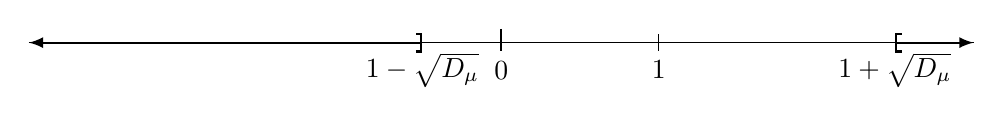
\begin{tikzpicture}
      \draw[] (-6, 0) -- (6, 0);
      \draw[{latex-]}, thick] (-6, 0) -- (-1, 0) node[below]{$1 - \sqrt{D_\mu}$};
      \draw[{latex-]}, thick] (6, 0) -- (5, 0) node[below]{$1 + \sqrt{D_\mu}$};
      \draw[thick] (0, 5pt) -- (0, -3pt) node[below]{$0$};
      \draw[] (2, 3pt) -- (2, -3pt) node[below]{$1$};
    \end{tikzpicture}
    \caption{Range of $m_1 / (\mu - a_2)$ in case 1.}
  \end{figure}

  Since neighborhood of $0$ is excluded in the range,
  there are only finite possibilities of $m_1$.
  Thus, $m_1$ can be decided.
\end{acase}

\begin{acase}{$D_\mu < 1$}
  WLOG $A_\mu (m_1) \leq B_\mu (m_4)$, then $A_\mu (m_1) \leq \sqrt{D_\mu} < 1$.
  This gives the bounds
  \[
    0 < 1 - \sqrt{D_\mu} \leq \frac{m_1}{\mu - a_2} \leq 1 + \sqrt{D_\mu}.
  \]
  \begin{figure}[!h]
    \centering
    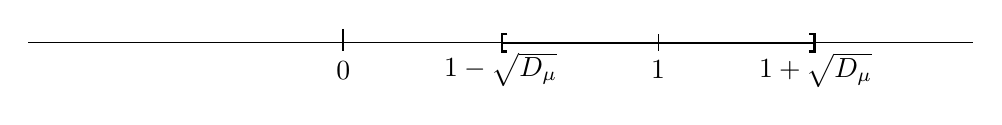
\begin{tikzpicture}
      \draw[] (-4, 0) -- (8, 0);
      \draw[] (2, 0) -- (2, 0) node[below]{$1 - \sqrt{D_\mu}$};
      \draw[{[-]}, thick] (2, 0) -- (6, 0) node[below]{$1 + \sqrt{D_\mu}$};
      \draw[thick] (0, 5pt) -- (0, -3pt) node[below]{$0$};
      \draw[] (4, 3pt) -- (4, -3pt) node[below]{$1$};
    \end{tikzpicture}
    \caption{Range of $m_1 / (\mu - a_2)$ in case 2.}
  \end{figure}

  Specifically, we obtain a lower bound $m_1 \geq (1 - \sqrt{D_\mu}) (\mu - a_2)$,
  within which there are only finitely many possible candidates.
  Hence, we can decide $m_1$.
\end{acase}

After $m_1, m_2, m_3$ are decided, $m_4$ can be computed from linear equation
\[
  \mu - m_3 - m_4 = \frac{m_2 m_3}{\mu - m_1 - m_2}.
\]
Recall that
\[
  \begin{array}{cccc}
    m_1 = \frac{1}{n_1 n_2}, & m_2 = \frac{1}{n_2 n_3},
    & m_3 = \frac{1}{n_3 n_4}, & m_4 = \frac{1}{n_4 n_5}
  \end{array}
\]
so there are finitely many candidates for $n_1, \cdots, n_5$.
Consequently, we can determine if such $m_1, \cdots, m_4$ admits such $\mathbf{n}$,
which completes the algorithm.

\end{document}
